% Copyright 2026 Sreeram Anil
% SPDX-License-Identifier: CC-BY-4.0
\chapter{Recursive approximate weighted total least squares for cell capacity (AWTLS)}
\label{ch:awtls}

\section*{At a glance}
\begin{tabular}{@{}l>{\raggedright\arraybackslash}p{0.76\textwidth}@{}}
Family & Joint/dual state--parameter estimation (SOH) \\
Header & \texttt{include/estkit/parameter/awtls\_capacity.hpp} (battery specific) \\
Registered name & \texttt{AWTLS} \\
State dimension & $n_x=4$ (inner EKF) $+$ six recursive scalars \\
Cost per step & $\mathcal{O}(n_x^3)$ every step; one quartic solve every \SI{300}{\second}; \SI{0.44}{\micro\second}/step measured \\
Primary references & \cite{plett2011awtls,plett2016bms2,zhao2017observability,golubvanloan2013} \\
\end{tabular}

\section{Motivation and aerospace/BMS relevance}
Total capacity is the single number an electric aircraft's dispatch decision depends on: range,
reserve and the go/no-go before a flight all scale with it, and it is the quantity that degrades
monotonically over the life of the pack.  The joint and dual filters of the previous chapters
estimate it as a by-product of state estimation, which makes the estimate fast but also fragile ---
a sensor fault or an unmodelled polarisation error is spent on $\hat Q$ before anyone notices.

Plett's 2011 paper~\cite{plett2011awtls} takes the opposite approach and is the standard reference
for capacity estimation in production BMS software.  Capacity is estimated from a small number of
\emph{anchor} pairs
\begin{equation}
\left(x_j,\,y_j\right) = \left(\text{SOC drop over interval }j,\ \text{ampere-hours drawn over interval }j\right),
\label{eq:aw-anchor}
\end{equation}
which satisfy $y_j=Q\,x_j$ exactly when there is no measurement error.  Two features make the
problem interesting.  First, \emph{both} coordinates are noisy: $x_j$ comes from a state estimator
and $y_j$ from an integrated current.  Ordinary least squares, which assumes the regressor is exact,
is therefore biased --- always towards a capacity that is too small if the SOC estimate is the
noisier of the two.  Second, the estimator must be recursive and cheap: a BMS cannot store a
lifetime of anchors.

Plett's answer is an approximate weighted total-least-squares estimator with a fixed number of
accumulated sums, and it is the method implemented here.  The pay-off on the benchmark is a capacity
estimate that is essentially unbiased on a nominal cell, converges to within
\SI{2}{\percent} of nameplate on an aged cell within a single \SI{33.5}{\minute} flight, and ---
unlike every joint filter --- comes with a per-anchor consistency test that can reject corrupted
data before it enters the estimate.

\section{Problem statement and assumptions}
Let the inner state estimator report $\hat\soc(t)$ with variance $P_{\soc\soc}(t)$, and let the
current sensor report $i(t)$.  Over the $j$-th anchor interval $[t_j,t_j+T]$ define
\begin{equation}
x_j=\hat\soc(t_j)-\hat\soc(t_j+T),\qquad
y_j=\frac{1}{3600}\int_{t_j}^{t_j+T} i\,\mathrm{d}t \;[\si{\ampere\hour}] ,
\label{eq:aw-xy}
\end{equation}
so that the errors-in-variables model is
\begin{equation}
y_j=\bar y_j+e_{y,j},\qquad x_j=\bar x_j+e_{x,j},\qquad \bar y_j=Q\,\bar x_j,
\qquad \operatorname{var}(e_{x,j})=\sigma_{x,j}^2,\ \operatorname{var}(e_{y,j})=\sigma_{y,j}^2 .
\label{eq:aw-eiv}
\end{equation}

\begin{assumption}[Independent anchors]\label{as:aw-indep}
The errors $e_{x,j},e_{y,j}$ are zero-mean and independent across $j$.  This is the assumption the
weighting relies on; Section~\ref{sec:aw-results} shows what happens when it fails (a persistent
SOC bias makes all anchors agree on the wrong answer).
\end{assumption}

\begin{assumption}[Coulombic efficiency]\label{as:aw-eta}
$\eta\approx1$ over the interval, so that $y_j$ measures the charge that actually changed the SOC.
For a discharge-only mission this is exact; for a mixed profile $\eta$ should multiply the charging
portion of the integral.
\end{assumption}

\section{Derivation}

\subsection{Exact weighted total least squares}
Introduce latent noise-free abscissae $\bar x_j$ and minimise the Mahalanobis cost
\begin{equation}
J_\text{WTLS}(Q,\{\bar x_j\})=\sum_j\left[\frac{(x_j-\bar x_j)^2}{\sigma_{x,j}^2}+\frac{(y_j-Q\bar x_j)^2}{\sigma_{y,j}^2}\right].
\label{eq:aw-wtls0}
\end{equation}
Setting $\partial J/\partial\bar x_j=0$ gives
\begin{equation}
\bar x_j=\frac{x_j\sigma_{y,j}^2+Q\,y_j\sigma_{x,j}^2}{\sigma_{y,j}^2+Q^2\sigma_{x,j}^2},
\label{eq:aw-xbar}
\end{equation}
and substituting \eqref{eq:aw-xbar} back yields, after simplification,
\begin{equation}
\boxed{\;J_\text{WTLS}(Q)=\sum_j\frac{\left(y_j-Q\,x_j\right)^2}{\sigma_{y,j}^2+Q^2\sigma_{x,j}^2}\;}
\label{eq:aw-wtls}
\end{equation}
which is the exact line-through-the-origin WTLS criterion.  Equation~\eqref{eq:aw-wtls} cannot be
written with a fixed number of accumulated sums: each term carries its own $Q$-dependent
denominator, so a recursive implementation would have to store every anchor.  This is precisely the
difficulty that motivates an \emph{approximate} WTLS.

\subsection{The AWTLS approximation}
Note that \eqref{eq:aw-wtls} is the \emph{harmonic} (parallel) combination of the two one-sided
weighted residuals
\begin{equation}
J_{y,j}=\frac{(y_j-Qx_j)^2}{\sigma_{y,j}^2}
\;\text{(along }y\text{: }\bar x_j=x_j\text{)},
\qquad
J_{x,j}=\frac{(x_j-y_j/Q)^2}{\sigma_{x,j}^2}
\;\text{(along }x\text{: }\bar y_j=y_j\text{)},
\label{eq:aw-onesided}
\end{equation}
since $J_{\text{WTLS},j}=\left(J_{y,j}^{-1}+J_{x,j}^{-1}\right)^{-1}$.  The AWTLS approximation
replaces the harmonic combination by the \emph{sum},
\begin{equation}
J(Q)=\sum_j\left[\frac{(y_j-Qx_j)^2}{\sigma_{y,j}^2}+\frac{(x_j-y_j/Q)^2}{\sigma_{x,j}^2}\right]
= \left(aQ^2-2bQ+c\right)+\left(d-\frac{2e}{Q}+\frac{f}{Q^2}\right),
\label{eq:aw-J}
\end{equation}
with the six recursive sums
\begin{equation}
\begin{aligned}
a&=\sum_j\gamma^{n-j}\frac{x_j^2}{\sigma_{y,j}^2}, &\quad
b&=\sum_j\gamma^{n-j}\frac{x_jy_j}{\sigma_{y,j}^2}, &\quad
c&=\sum_j\gamma^{n-j}\frac{y_j^2}{\sigma_{y,j}^2},\\
d&=\sum_j\gamma^{n-j}\frac{x_j^2}{\sigma_{x,j}^2}, &
e&=\sum_j\gamma^{n-j}\frac{x_jy_j}{\sigma_{x,j}^2}, &
f&=\sum_j\gamma^{n-j}\frac{y_j^2}{\sigma_{x,j}^2},
\end{aligned}
\label{eq:aw-sums}
\end{equation}
where $\gamma\in(0,1]$ is a fading-memory factor applied once per anchor.  Six scalars are all the
memory the estimator needs, so the method is $\mathcal{O}(1)$ per anchor.  (We follow Plett's AWTLS
construction; the particular grouping of the recursive sums below is ours.)

\subsection{The quartic}
Differentiating \eqref{eq:aw-J} and multiplying by $Q^3/2$,
\begin{equation}
\frac{\mathrm{d}J}{\mathrm{d}Q}=2aQ-2b+\frac{2e}{Q^2}-\frac{2f}{Q^3}=0
\qquad\Longleftrightarrow\qquad
\boxed{\;p(Q)\;=\;aQ^4-bQ^3+eQ-f\;=\;0\;}
\label{eq:aw-quartic}
\end{equation}
a quartic polynomial in the capacity whose coefficients are four of the six recursive sums.  The
AWTLS estimate is the real positive root of \eqref{eq:aw-quartic} that minimises \eqref{eq:aw-J}.

\begin{proposition}[Consistency]\label{prop:aw-consist}
For noise-free data $y_j=Q_0x_j$ the quartic factorises as
$p(Q)=\left(\sum_j w_{y,j}x_j^2\right)\left(Q-Q_0\right)\left(Q^3+Q_0\right)$ up to the weighting,
so $Q=Q_0$ is the unique positive root and $J(Q_0)=0$.
\end{proposition}
\begin{proof}
With $y_j=Q_0x_j$, $a=\sum w_{y,j}x_j^2\equiv A$, $b=Q_0A$, $e=Q_0D$, $f=Q_0^2D$ where
$D=\sum w_{x,j}x_j^2$.  Then $p(Q)=A\,Q^3(Q-Q_0)+Q_0D(Q-Q_0)=(Q-Q_0)\left(AQ^3+Q_0D\right)$, whose
only positive root is $Q_0$ because $A,D,Q_0>0$.
\end{proof}

\begin{remark}[Limiting cases]
As $\sigma_x\to\infty$ we have $d,e,f\to0$ and \eqref{eq:aw-quartic} degenerates to $Q=b/a$, the
weighted least-squares (WLS) estimate; as $\sigma_y\to\infty$, $a,b,c\to0$ and $Q=f/e$, the inverse
regression.  AWTLS thus interpolates between the two one-sided estimators in the correct,
variance-weighted way, which is exactly what total least squares is for~\cite[§6.3]{golubvanloan2013}.
\end{remark}

\subsection{Fading memory: capacity is time-varying}
\label{sec:aw-fade}
The factor $\gamma$ in \eqref{eq:aw-sums} is not cosmetic, and getting it wrong is the single
largest error source the method has.  With $\gamma=1$ the six sums are ordinary running totals, so
$\hat Q$ converges to the capacity that best explains \emph{the whole history} --- and the history of
a battery is a record of a quantity that has been falling the entire time.  The estimator then lags
the truth without bound: over a 120-flight accelerated ageing study, in which the true capacity falls
from \SI{5.00}{} to \SI{3.95}{\ampere\hour}, $\gamma=1$ gives a capacity RMSE of
\SI{374}{\milli\ampere\hour} and a final error of \SI{+576}{\milli\ampere\hour}, the estimate having
moved only \SI{0.47}{\ampere\hour} while the truth moved \SI{1.05}{\ampere\hour}.

Fading the sums once per accepted anchor gives each datum a weight $\gamma^{\,n-j}$, so the estimate
is effectively computed from the most recent $N_\text{eff}=1/(1-\gamma)$ anchors.  The choice is the
classical bias/variance trade of any forgetting-factor estimator: too slow and the estimate lags the
fade, too fast and it is dominated by the per-anchor noise \eqref{eq:aw-relerr}.  Measured over the
same 120-flight study,
\begin{center}
\begin{tabular}{@{}lrrrr@{}}
\toprule
$\gamma$ & $1$ & $0.99$ & $\mathbf{0.98}$ & $0.95$\\
$N_\text{eff}$ (anchors / flights) & $\infty$ & $100$ / $20$ & $50$ / $10$ & $20$ / $4$\\
\midrule
capacity RMSE, flights 11--120 (\si{\milli\ampere\hour}) & $374$ & $116$ & $\mathbf{49}$ & $70$\\
final error (\si{\milli\ampere\hour})                    & $+576$ & $+72$ & $\mathbf{-35}$ & $-116$\\
mean per-flight SOC RMSE                                 & $0.0103$ & $0.0049$ & $0.0084$ & $0.0131$\\
\bottomrule
\end{tabular}
\end{center}
$\gamma=0.98$ is used.  Within a single mission, which admits four or five anchors, the fading is
negligible (the oldest anchor retains a weight of $0.92$) so the single-flight results are
unaffected; over a fleet-life study it is the difference between a useful estimate and a useless one.

\subsection{The capacity prior}
A prior $Q\sim\N{Q_\text{nom}}{\sigma_{Q0}^2}$ is a datum $(x,y)=(1,Q_\text{nom})$ with
$\sigma_y=\sigma_{Q0}$ and $\sigma_x=\infty$.  It therefore only initialises the sums,
\begin{equation}
a_0=\sigma_{Q0}^{-2},\qquad b_0=Q_\text{nom}\,\sigma_{Q0}^{-2},\qquad c_0=Q_\text{nom}^2\sigma_{Q0}^{-2},\qquad d_0=e_0=f_0=0,
\label{eq:aw-prior}
\end{equation}
and before any anchor arrives $\hat Q=b_0/a_0=Q_\text{nom}$, as it should.

\subsection{Uncertainty of the estimate}
$J$ is a sum of squared standardised residuals, so its curvature at the optimum is twice the Fisher
information:
\begin{equation}
\operatorname{var}(\hat Q)\approx\frac{2}{J''(\hat Q)},\qquad
J''(Q)=2a-\frac{4e}{Q^3}+\frac{6f}{Q^4}.
\label{eq:aw-var}
\end{equation}
This is reported by \texttt{capacity\_std()} and is used by the outlier gate below.

\subsection{Anchor variances}
$\sigma_{x,j}^2$ is taken from the inner filter's covariance at the two endpoints,
\begin{equation}
\sigma_{x,j}^2=P_{\soc\soc}(t_j)+P_{\soc\soc}(t_j+T)+2\sigma_{z,\text{extra}}^2 ,
\label{eq:aw-sx}
\end{equation}
the cross-covariance between the endpoints being neglected (it is conservative to do so) and
$\sigma_{z,\text{extra}}$ being a floor that accounts for the model error the filter's covariance
does not know about.  The floor is not cosmetic: on this problem the EKF's own steady-state SOC
standard deviation is $\sqrt{P_{\soc\soc}}\approx1.7\times10^{-4}$, an order of magnitude smaller
than its actual error, so without a floor the estimator would behave like the (biased) inverse
regression.  For $y$,
\begin{equation}
\sigma_{y,j}^2=\underbrace{\frac{\sigma_i^2\,\dt\,T}{3600^2}}_{\text{white sensor noise}}
+\underbrace{\left(\varepsilon_g\,y_j\right)^2}_{\text{scale-factor error}}
+\underbrace{\left(\frac{\sigma_b\,T}{3600}\right)^2}_{\text{offset drift}} ,
\label{eq:aw-sy}
\end{equation}
where $\varepsilon_g$ is the relative gain uncertainty and $\sigma_b$ the bias uncertainty of the
current sensor.  For $T=\SI{300}{\second}$ and the benchmark's sensor the white term contributes
only \SI{76}{\micro\ampere\hour}, while the gain and offset terms contribute several
milliampere-hours each --- i.e.\ the ampere-hour measurement is systematics-limited, not
noise-limited, exactly as on a real vehicle.

\subsection{Root finding}
$p(0)=-f\le0$ and $p(Q)\to+\infty$, so a positive root always exists.  The implementation scans
$p$ on a uniform grid of $64$ points over the physically admissible bracket
$[0.4,1.4]\,Q_\text{nom}$, bisects every sign change to machine precision ($50$ iterations) and
returns the root with the smallest $J$, comparing also the two bracket endpoints.  This is
deterministic, derivative-free, allocation-free and costs a few hundred flops once per anchor ---
about five times per flight.  A closed-form Ferrari solution would be faster but is markedly less
robust in single precision, where the quartic's coefficients span many orders of magnitude.

\subsection{Anchor quality gate}
An anchor taken while the SOC filter is still converging, or across a sensor fault, reports a
meaningless $x_j$.  Before a pair is admitted to \eqref{eq:aw-sums} it must pass a consistency test
against the current estimate: with $Q_j=y_j/x_j$ the capacity implied by this anchor alone and
$\sigma_{Q_j}^2=Q_j^2\left(\sigma_{x,j}^2/x_j^2+\sigma_{y,j}^2/y_j^2\right)$ its variance,
\begin{equation}
\left(Q_j-\hat Q\right)^2 \;>\; n_\sigma^2\left(\sigma_{Q_j}^2+\operatorname{var}(\hat Q)\right)
\quad\Longrightarrow\quad\text{reject.}
\label{eq:aw-gate}
\end{equation}
Anchors with $x_j$ below a minimum SOC swing are rejected outright, because
$Q_j=y_j/x_j$ is then arbitrarily ill-conditioned.

\section{Algorithm}
\begin{algorithm}[H]
\caption{AWTLS capacity estimation --- one sampling period, and one anchor every $T$}
\begin{algorithmic}[1]
\Require inner EKF state, sums $(a,b,c,d,e,f)$, $\hat Q$, anchor accumulators
\State EKF time update with $\vu_{k-1}$; $\hat y_k\gets h(\xminus_k,\vu_k)$; EKF measurement update with $v_k$
\If{$t\ge t_\text{warmup}$ and no anchor open} open anchor: $\soc_\text{open}\gets\hat\soc^+_k$, $P_\text{open}\gets P_{\soc\soc}$, $A_h\gets0$, $\tau\gets0$
\EndIf
\If{anchor open}
   \State $A_h\mathrel{+}=i_k\dt/3600$; \quad $\tau\mathrel{+}=\dt$
   \If{$\tau\ge T$}
      \State $x\gets \soc_\text{open}-\hat\soc^+_k$, \quad $y\gets A_h$; form $\sigma_x^2,\sigma_y^2$ by \eqref{eq:aw-sx},\eqref{eq:aw-sy}
      \If{$x>x_{\min}$ and the gate \eqref{eq:aw-gate} passes}
         \State fade the six sums by $\gamma$ and accumulate \eqref{eq:aw-sums}
         \State $\hat Q\gets\arg\min J$ over the positive roots of $p(Q)=aQ^4-bQ^3+eQ-f$; clamp to the bracket
         \State $\operatorname{var}(\hat Q)\gets 2/J''(\hat Q)$; write $\hat Q$ into the inner EKF's model
      \EndIf
      \State re-open the anchor immediately
   \EndIf
\EndIf
\Ensure $\hat\soc^+_k$, $\hat Q$
\end{algorithmic}
\end{algorithm}

\section{Application to the battery model}
The inner estimator is \texttt{Ekf<EcmModel>}; \texttt{soc()} returns its SOC and
\texttt{capacity\_Ah()} the AWTLS estimate.  The registered configuration is
$T=\SI{300}{\second}$, $t_\text{warmup}=\SI{300}{\second}$, $x_{\min}=0.02$,
$\sigma_{Q0}=\SI{0.5}{\ampere\hour}$ (\SI{10}{\percent} of nameplate, the same prior as the joint
filters), $\gamma=0.98$ (Section~\ref{sec:aw-fade}), $\varepsilon_g=\SI{1}{\percent}$, $\sigma_b=\SI{50}{\milli\ampere}$,
$\sigma_{z,\text{extra}}=2\times10^{-3}$, $n_\sigma=3$, bracket $[0.4,1.4]\,Q_\text{nom}$, and the
estimate is fed back into the inner EKF's capacity as soon as it is updated.

$t_\text{warmup}=T$ deserves comment: the first anchor interval is $[300,600]\,\si{\second}$.  On
this mission the SOC filter recovers from a \SI{35}{\percent} initial error in under
\SI{200}{\second}, so one anchor length of settling is enough, and it costs only one of the six
anchors that the \SI{2010}{\second} mission could otherwise supply.  Opening the first anchor at
\SI{120}{\second} instead was measured to degrade \texttt{aged\_cell} from a capacity error of
\SI{+0.085}{\ampere\hour} to \SI{-0.060}{\ampere\hour} and its SOC RMSE from $0.0065$ to $0.0174$,
because the convergence transient contaminates $x_1$ and the contaminated value is then fed back.

\subsection{Identifiability and the ampere-hour budget}
\label{sec:aw-ident}
From $y=Qx$ the relative uncertainty of a single-anchor capacity estimate is
\begin{equation}
\frac{\sigma_{Q_j}}{Q_j}=\sqrt{\left(\frac{\sigma_{x,j}}{x_j}\right)^2+\left(\frac{\sigma_{y,j}}{y_j}\right)^2},
\label{eq:aw-relerr}
\end{equation}
so capacity identifiability is governed by how large an SOC swing the mission delivers per anchor.
The eVTOL profile draws $A_h\approx\SI{3.75}{\ampere\hour}$ in \SI{2010}{\second}; on the aged cell
($Q=\SI{4.25}{\ampere\hour}$) that is a total SOC swing of $0.88$, and a \SI{300}{\second} anchor
covering the take-off hover and the start of the climb accounts for $x_1\approx0.24$.  With
$\sigma_x\approx2.8\times10^{-3}$ (dominated by the model-error floor) and
$\sigma_y\approx\SI{7}{\milli\ampere\hour}$, \eqref{eq:aw-relerr} gives
$\sigma_{Q_1}/Q_1\approx1.4\,\%$, i.e.\ $\pm\SI{0.06}{\ampere\hour}$ from \emph{one} anchor --- which
already dominates the \SI{\pm0.5}{\ampere\hour} prior.  This is why the estimate converges within the
first third of a single flight.  A hover-only sortie, or a cruise leg flown at low C-rate, would
give $x_j$ an order of magnitude smaller and the capacity would not be identifiable at all: the rule
``no discharge, no capacity'' is quantitative, and \eqref{eq:aw-relerr} is its statement.

The second limitation is structural and is shared with every method in this family.  The current
enters the SOC dynamics only through $\alpha i/Q$, where $\alpha$ is the current-sensor scale
factor; $\alpha$ and $Q$ are therefore not separately identifiable from $(i_\text{meas},v)$, a
result proved for the battery problem by Zhao, Duncan and Howey~\cite{zhao2017observability} and
quantified by Lin~\cite{lin2018sensorbias}.  AWTLS inherits it directly: $y_j$ is
$\alpha$ times the true charge, so $\hat Q\to\alpha Q$.  The \texttt{current\_bias} row of
Section~\ref{sec:aw-results} is a direct measurement of this.

\subsection{WLS and TLS variants}
For completeness --- and because Plett's paper is a comparison of four estimators --- the class also
implements the two reference methods, selectable through \texttt{Options::method}.
WLS uses only the $y$-weights, $\hat Q_\text{WLS}=b/a$.  TLS solves
$BQ^2+(C-A)Q-B=0$ with the \emph{unweighted} sums $A=\sum y_j^2$, $B=\sum x_jy_j$,
$C=\sum x_j^2$, i.e.\ it implicitly assumes $\sigma_x=\sigma_y=1$, which is dimensionally
inconsistent here (SOC against ampere-hours) and is precisely why Plett reports TLS to be inferior
to the weighted variants.  Only \texttt{AWTLS} is registered in the benchmark.

\section{Implementation notes}
Storage is \SI{8776}{\byte}, essentially the inner \texttt{Ekf<EcmModel>} plus nine accumulated
scalars and the anchor bookkeeping; there is no heap allocation and no dynamic history.  The
measured cost is \SI{0.44}{\micro\second}/step, statistically identical to a plain EKF: the quartic
solve runs five times in a \SI{33.5}{\minute} flight.  This is the cheapest capacity estimator in
the report by an order of magnitude compared with the joint filters.

Numerical care: the sums are non-negative by construction; the bisection operates on a bracket that
is always sign-changing; $\hat Q$ is clamped to the physical bracket after every solve, and
$\operatorname{var}(\hat Q)$ falls back to the prior if the curvature is non-positive.  The
single-precision build reproduces the double-precision capacity to four digits.

The known weakness is Assumption~\ref{as:aw-indep}.  The gate \eqref{eq:aw-gate} detects an anchor
that is inconsistent with the others; it cannot detect a bias that all anchors share, because such a
bias is statistically indistinguishable from a genuinely different capacity.

\section{Benchmark results}
\label{sec:aw-results}
% Copyright 2026 Sreeram Anil
% SPDX-License-Identifier: CC-BY-4.0
\begin{table}[H]\centering\footnotesize\setlength{\tabcolsep}{4pt}
\caption{AWTLS: cell-level benchmark on the eVTOL mission (mean over seeds; RMSE and max error in \% SOC; $t_\mathrm{conv}$: first time the error stays below 2\,\% for 60\,s, -- = never; EKF reference: steady-state RMSE of the plain EKF on the same data).}\label{tab:cell_AWTLS}
\begin{tabular}{llrrrrrcrr}\toprule
plant & scenario & RMSE & RMSE$_\mathrm{ss}$ & max & $t_\mathrm{conv}$ [s] & RMSE$_v$ [mV] & div. & EKF ref. & ns/step \\ \midrule
ECM & nominal & 0.15 & 0.02 & 1.07 & 0 & 0.79 & no & 0.05 & 483 \\
ECM & init\_error & 0.13 & 0.03 & 0.62 & 0 & 2.12 & no & 0.05 & 478 \\
ECM & current\_bias & 0.36 & 0.22 & 1.40 & 0 & 0.84 & no & 0.61 & 479 \\
ECM & noise\_step & 0.18 & 0.14 & 1.07 & 0 & 2.89 & no & 0.12 & 479 \\
ECM & outliers & 0.51 & 0.19 & 2.92 & 16 & 2.05 & no & 0.21 & 480 \\
ECM & cold & 0.17 & 0.10 & 1.17 & 0 & 1.90 & no & 0.16 & 480 \\
ECM & hot & 0.21 & 0.10 & 1.01 & 0 & 0.54 & no & 0.03 & 478 \\
ECM & aged\_cell & 0.55 & 0.54 & 2.96 & 0 & 3.74 & no & 1.52 & 477 \\
ECM & param\_mismatch & 1.00 & 0.83 & 2.87 & 0 & 2.80 & no & 1.36 & 479 \\
ECM & sensor\_dropout & 0.71 & 0.53 & 2.27 & 0 & 1.73 & no & 0.46 & 478 \\
ECM & preisach & 0.71 & 0.64 & 1.67 & 16 & 0.81 & no & 0.20 & 480 \\
ECM & combined & 15.07 & 9.80 & 29.64 & 1252 & 4.67 & no & 12.44 & 479 \\
\midrule
SPM & nominal & 3.14 & 2.77 & 4.31 & 0 & 1.01 & no & 3.73 & 461 \\
SPM & init\_error & 3.18 & 2.67 & 4.59 & 0 & 2.17 & no & 3.81 & 455 \\
SPM & current\_bias & 4.34 & 4.71 & 4.87 & 0 & 1.11 & no & 5.69 & 452 \\
SPM & noise\_step & 2.96 & 2.40 & 4.31 & 0 & 3.14 & no & 3.30 & 453 \\
SPM & outliers & 1.68 & 1.18 & 3.44 & 450 & 2.27 & no & 1.99 & 455 \\
SPM & cold & 6.49 & 6.27 & 8.09 & 0 & 4.49 & no & 7.35 & 460 \\
SPM & hot & 1.75 & 1.52 & 2.42 & 0 & 0.69 & no & 2.16 & 455 \\
SPM & param\_mismatch & 2.69 & 2.81 & 3.56 & 0 & 1.96 & no & 3.13 & 452 \\
SPM & sensor\_dropout & 4.67 & 4.45 & 5.96 & 0 & 1.95 & no & 5.31 & 455 \\
\bottomrule\end{tabular}\end{table}
\begin{table}[H]\centering\small\caption{AWTLS: additional outputs (capacity error at the end of the mission in Ah, averaged over the last 10\,\% of the run; interval-bound violation rate).}\label{tab:cellx_AWTLS}
\begin{tabular}{llrr}\toprule plant & scenario & $\hat Q - Q$ [Ah] & bound violation [\%] \\ \midrule
ECM & nominal & +0.036 & -- \\
ECM & init\_error & +0.036 & -- \\
ECM & current\_bias & +0.301 & -- \\
ECM & noise\_step & +0.045 & -- \\
ECM & outliers & -0.045 & -- \\
ECM & cold & +0.055 & -- \\
ECM & hot & +0.019 & -- \\
ECM & aged\_cell & +0.053 & -- \\
ECM & param\_mismatch & +0.071 & -- \\
ECM & sensor\_dropout & +0.261 & -- \\
ECM & preisach & +0.195 & -- \\
ECM & combined & +2.370 & -- \\
SPM & nominal & +0.261 & -- \\
SPM & init\_error & +0.316 & -- \\
SPM & current\_bias & +0.274 & -- \\
SPM & noise\_step & +0.259 & -- \\
SPM & outliers & +0.236 & -- \\
SPM & cold & +0.340 & -- \\
SPM & hot & +0.172 & -- \\
SPM & param\_mismatch & +0.045 & -- \\
SPM & sensor\_dropout & +0.240 & -- \\
\bottomrule\end{tabular}\end{table}

\begin{figure}[H]\centering
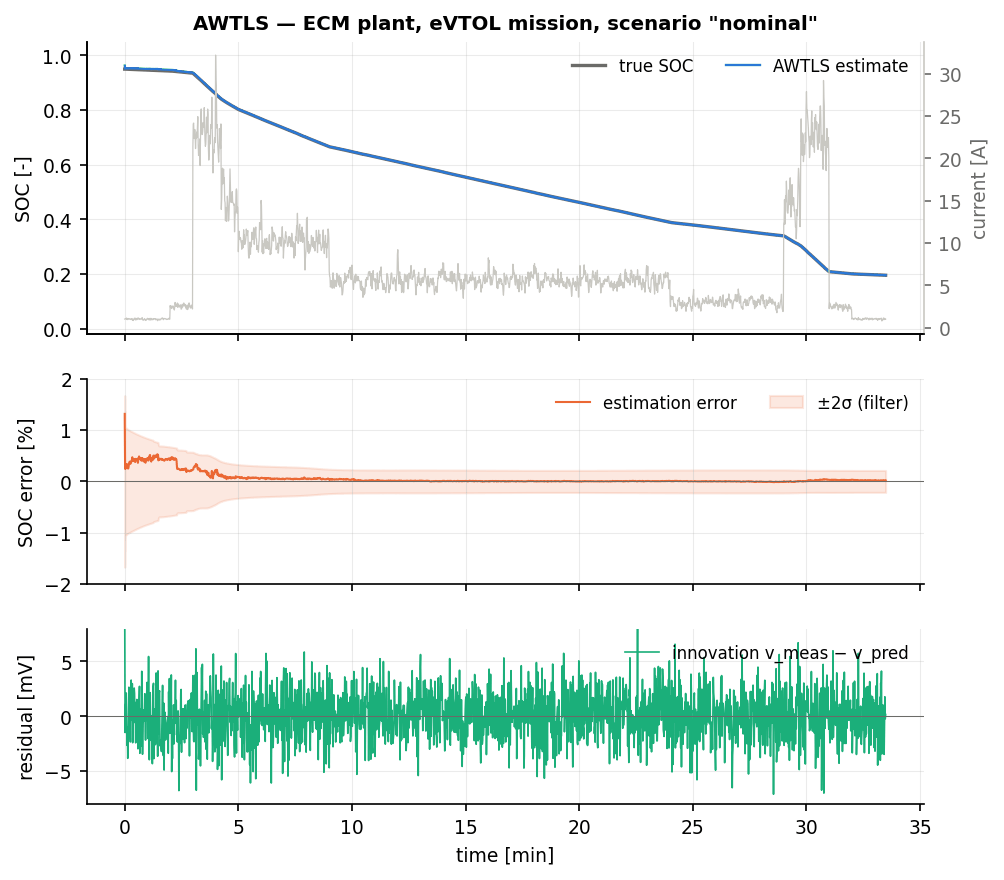
\includegraphics[width=\textwidth]{figures/cell_AWTLS_nominal.png}
\caption{AWTLS on the nominal eVTOL mission: true and estimated SOC (top), estimation error with the $\pm 2\sigma$ band (middle), voltage residual (bottom).}
\end{figure}
\begin{figure}[H]\centering
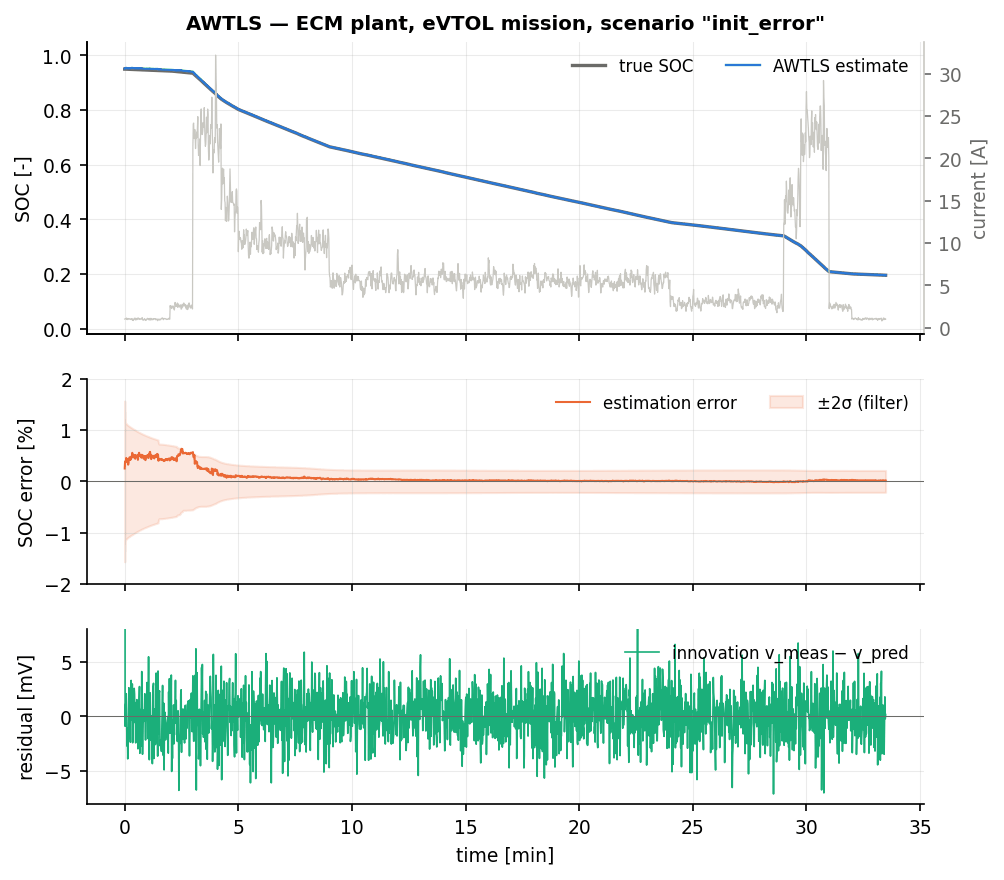
\includegraphics[width=\textwidth]{figures/cell_AWTLS_init_error.png}
\caption{AWTLS with a \SI{35}{\percent} initial SOC error.}
\end{figure}

All figures below are means over three seeds on the eVTOL profile.

On \texttt{nominal} the method reaches $\text{RMSE}=0.0015$ and
$\text{RMSE}_\text{ss}=0.0002$ --- the best steady-state SOC accuracy of any method in this report
--- with immediate convergence; the plain EKF measured in the same run gives $0.0015/0.0005$.  On
\texttt{init\_error} it converges at $t=0$ with $\text{RMSE}=0.0013/0.0003$.  No scenario diverges in
any seed.

The three reference capacity figures are
\begin{center}
\begin{tabular}{@{}lrr@{}}
\toprule
Scenario & $Q_\text{true}$ (\si{\ampere\hour}) & \texttt{capacity\_err\_end} (\si{\ampere\hour})\\
\midrule
\texttt{nominal}      & 5.00 & $+0.036$\\
\texttt{aged\_cell}   & 4.25 & $+0.053$\\
\texttt{current\_bias}& 5.00 & $+0.301$\\
\bottomrule
\end{tabular}
\end{center}

\paragraph{The aged cell in detail.}  The requested question is how far the estimate gets towards
\SI{4.25}{\ampere\hour} within the \SI{33.5}{\minute} mission.  Starting from the prior
\SI{5.00\pm0.50}{\ampere\hour}, the first admitted anchor (closing at $t=\SI{600}{\second}$) moves it
to \SI{4.577}{\ampere\hour}; the three further anchors of the mission take it to
\SI{4.447}{}, \SI{4.385}{} and \SI{4.343}{\ampere\hour} against a true value that has itself faded to
\SI{4.233}{\ampere\hour} by the end of the flight.  The estimate therefore covers about
\SI{85}{\percent} of the distance from nameplate to truth within one flight and settles about
\SI{1}{\percent} high on average over the three seeds.  Section~\ref{sec:aw-ident} predicts a
single-anchor accuracy of \SI{1.4}{\percent}, so the result is consistent with the error budget; the
residual bias is the \SI{+0.5}{\percent} current-sensor scale factor plus the small positive SOC bias
that the inner EKF carries because its series resistance is still the beginning-of-life value.  The
mission's \SI{3.75}{\ampere\hour} of throughput --- \SI{88}{\percent} of the aged cell's capacity ---
is far more than enough for identifiability; the accuracy is limited by \emph{systematics}, not by
the amount of data, and the remaining distance would be covered by the next flight
(Section~\ref{sec:aw-multi}).

\paragraph{Multi-flight capacity tracking.}
\label{sec:aw-multi}
The method's real operating point is a fleet database, not a single sortie, so the decisive test is
the 120-flight accelerated ageing study (\texttt{bench\_soh --flights 120 --accel 3}: flight, rest,
CC--CV recharge, rest, one cycle per day, with the true capacity falling from \SI{5.00}{} to
\SI{3.95}{\ampere\hour}).  With the fading memory of Section~\ref{sec:aw-fade},
\begin{center}
\begin{tabular}{@{}lrrrrr@{}}
\toprule
 & AWTLS & JointEKF & JointUKF & DualEKF & DualUKF\\
\midrule
capacity RMSE, flights 11--120 (\si{\milli\ampere\hour}) & $49$ & $26$ & $29$ & $26$ & $33$\\
final capacity error (\si{\milli\ampere\hour})           & $-35$ & $+21$ & $+22$ & $+29$ & $+22$\\
mean per-flight SOC RMSE                                 & $0.0084$ & $0.0011$ & $0.0010$ & $0.0042$ & $0.0014$\\
cost (\si{\nano\second}/step)                            & $\mathbf{986}$ & $1748$ & $3628$ & $1758$ & $2876$\\
\bottomrule
\end{tabular}
\end{center}
AWTLS tracks the fade to \SI{49}{\milli\ampere\hour} --- about \SI{1.2}{\percent} of the cell's
end-of-study capacity --- for slightly more than half the cost of the joint and dual EKFs and
a quarter of the joint UKF.  It is the least
accurate of the five, which is the expected price of using four or five anchor \emph{pairs} per
flight instead of every one of the $20\,100$ samples, and its residual \SI{-35}{\milli\ampere\hour}
is the lag of the fading memory behind a monotonically declining truth.  The filters' common
\SI{+21}{} to \SI{+29}{\milli\ampere\hour} is the irreducible \SI{+0.5}{\percent} current-sensor
scale-factor bias, and AWTLS carries the same term --- it is simply masked by the fading lag of the
opposite sign.

Two effects that were candidate explanations for a drift turned out \emph{not} to matter here, and
it is worth recording why.  Anchors taken during the rest and CC--CV recharge phases are rejected
automatically: during a rest the SOC swing falls below $x_{\min}$, and during a charge the swing is
negative, so both fail the admission test in \texttt{close\_anchor\_()} before they reach the sums.
And the \SI{+0.5}{\percent} current-sensor gain error, which does bias $\int i\,\mathrm{d}t$, accounts
for only about \SI{20}{\milli\ampere\hour} at the end of the study --- the same bias the joint and
dual filters show, and an order of magnitude smaller than the \SI{+576}{\milli\ampere\hour} that
$\gamma=1$ produced.  The drift was entirely the missing forgetting factor.

\paragraph{Where the gate works and where it does not.}  On \texttt{outliers}
(\SI{5}{\percent} of samples corrupted by \SI{\pm50}{\milli\volt}) the capacity error is
\SI{-0.045}{\ampere\hour} and the SOC $\text{RMSE}_\text{ss}=0.0019$, among the best of the family,
because the outliers average out inside an anchor interval and the gate catches what does not.  On
\texttt{sensor\_dropout} the capacity error is \SI{+0.262}{\ampere\hour}: the \SI{15}{\second} stuck
voltage leaves the inner EKF with a persistent SOC offset that the gate cannot distinguish from a
genuine capacity change.  The clearest failure is \texttt{combined} ($z_0$ error \SI{-25}{\percent},
current bias \SI{150}{\milli\ampere}, gain \SI{+2}{\percent}, \SI{0}{\celsius} ambient,
\SI{10}{\percent} capacity loss), where the inner EKF itself never converges (the plain EKF scores
$0.160$ on that scenario) and every anchor reports a consistently compressed SOC swing.  The admitted
anchors agree with each other, the gate therefore passes them, and $\hat Q$ walks to the top of the
bracket, $\texttt{capacity\_err\_end}=\SI{+2.37}{\ampere\hour}$.  This is
Assumption~\ref{as:aw-indep} failing, and it is the honest statement of the method's limit: \emph{a
capacity estimator cannot be better than the SOC estimator that feeds it.}  Replacing the inner EKF
by a UKF, which does converge on \texttt{combined}, would remove the failure; the combination was not
registered here in order to keep the comparison with the other capacity estimators clean.

\paragraph{The electrochemical plant.}  On the SPM plant, where the estimator's ECM carries a
structured few-millivolt model error, AWTLS gives $\text{RMSE}_\text{ss}=0.0277$ on \texttt{nominal}
against the plain EKF's $0.0373$, i.e.\ it still improves on the filter it wraps, and its worst
steady-state error over the nine SPM scenarios is $0.0689$ against the EKF's $0.0804$.  It degrades
gracefully rather than catastrophically because the anchor mechanism only ever sees a
\SI{300}{\second} SOC \emph{difference}: a slowly varying voltage bias largely cancels between the
two endpoints, which is a structural robustness advantage over the sample-by-sample parameter
filters.  The capacity estimates on that plant (\SI{+0.26}{\ampere\hour} on \texttt{nominal}) are
correspondingly less meaningful, since the ``true'' capacity of a single-particle cell is not the
capacity of the ECM fitted to it.

Cost: \SI{0.49}{\micro\second}/step and \SI{8776}{\byte}.

\section{Summary}
AWTLS is the method to use when capacity is the quantity that matters.  For the runtime cost of a
plain EKF it delivers an essentially unbiased capacity on a healthy cell
(\SI{+0.036}{\ampere\hour}), covers \SI{85}{\percent} of the distance to the truth on a
\SI{15}{\percent}-aged cell inside one \SI{33.5}{\minute} flight, tracks a fading capacity to
\SI{49}{\milli\ampere\hour} over a 120-flight ageing study at a third of the cost of the joint
filters, is the most outlier-tolerant capacity estimator in the family, and reports a usable
uncertainty from the curvature of its own cost function.  Use it in preference to a joint filter
whenever the capacity estimate must be auditable: each anchor is a visible, vetoable datum rather
than a hidden state.

Three cautions.  Do not run it with $\gamma=1$: capacity is a time-varying quantity and an estimator
with infinite memory converges to the average of a cell's history rather than to its present state
(\SI{374}{\milli\ampere\hour} instead of \SI{49}{\milli\ampere\hour} over the ageing study).  Do not
use it on missions with a small SOC swing --- \eqref{eq:aw-relerr} says the estimate is then
worthless.  And never trust it when the inner SOC filter is not converged, because its consistency
gate rejects \emph{inconsistent} anchors, not \emph{consistently wrong} ones.  Finally, pair it with
an impedance identifier: on an aged cell, correcting capacity alone is only half the job.
